%!TEX root = ../../../main.tex

	\section{Photon correlation measurements} \label{subsec::g2}

		The investigated \sivs exhibit count rates of a few thousand to a few \num{100000} counts per second (\SI{}{\cps}).
		We carried out measurements of the photon statistics and found that about \SI{3}{\percent} of luminescent \nds contain single color centers.
		These measurements show, that the probability of finding a single emitter does not correlate in any way with the \cwl or the \lw of the ZPL.
		We found several single \sivs with an anti-bunching dip down to about \num{0.2} and attribute the residual \gtz value to background fluorescence from the diamond host.
		For the utilized \nds a background measurement without simultaneously measuring \siv \pl is infeasible, because the laser spot size is bigger than the \nd, i.e.\ the \siv will always be excited when the \nd is illuminated.
		Therefore, the background is estimated from the sideband of \siv spectra.
		The measured lifetimes of the single \sivs are in the range of about \SIrange{1}{9}{\ns}, which is of the same order as previous research suggests \cite{Sipahigil2014,Sternschulte1994}.

		\Fref{fig::g2} shows the \gt functions of one emitter of \hl and one emitter of \vl.
		The former emitter's spectrum is shown in \Fref{subfig::erlangen_spectrum}, and denoted \emhtwo. The latter is the same as \embroad introduced in \Fref{sec::spectra}.

		\begin{figure}[!htb]
			\begin{subfigure}[tp]{ 0.49\linewidth}
				\centering
				\testbox{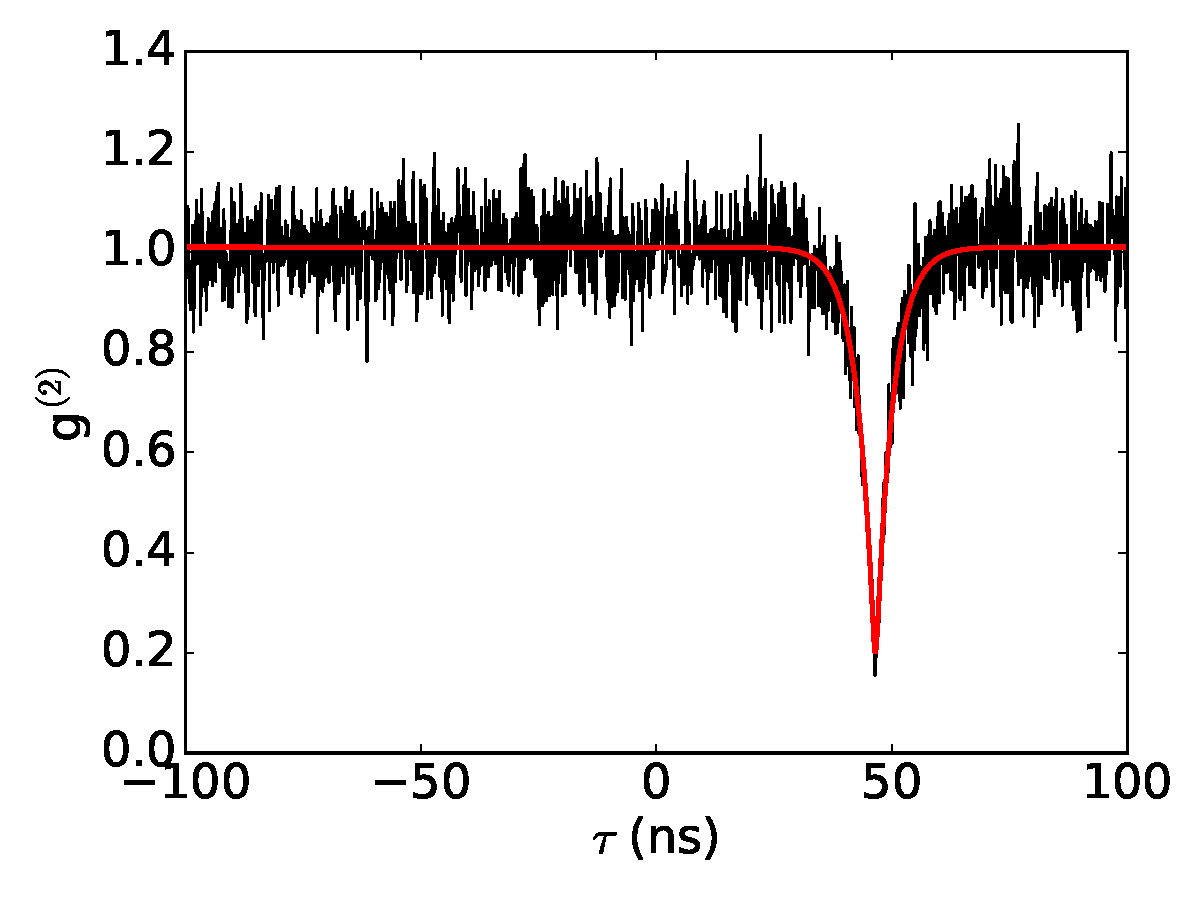
\includegraphics[trim = 0 0 0 0,  clip= true, width = \pairplotwide]{./pics/siv_sarah_g2_90k_2_notitle_original_fit.pdf}}
				\caption{}\label{subfig::g2_a}
			\end{subfigure}
			\hfill
			\begin{subfigure}[tp]{ 0.49\linewidth}
				\centering
				\testbox{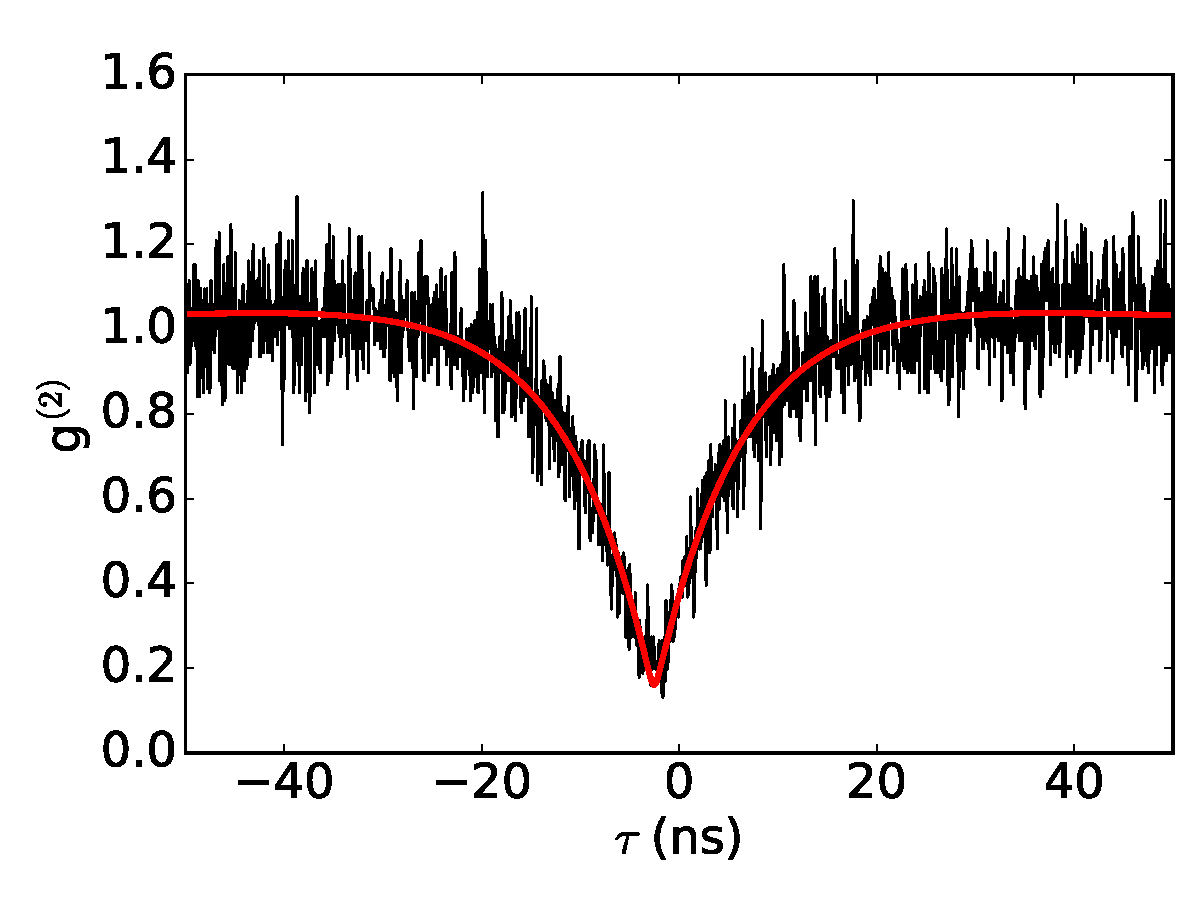
\includegraphics[trim = 0 0 0 0,  clip= true, width = \pairplotwide]{./pics/Ir8_g2_scan_xy-05_200uW_fit.pdf}}
				\caption{}\label{subfig::g2_b}
			\end{subfigure}
			\caption[Intensity autocorrelation measurements for \hl and \vl]{(a) Intensity autocorrelation function of an emitter in \hl. (b) Intensity autocorrelation function of \embroad at an excitation power of \SIlist{200}{\micro\W}. Saturation power is \SI{1}{mW}.}
			\label{fig::g2}
		\end{figure}

		\begin{figure}[!htb]
			\begin{subfigure}[t]{ 0.49\linewidth}
				\centering
				\testbox{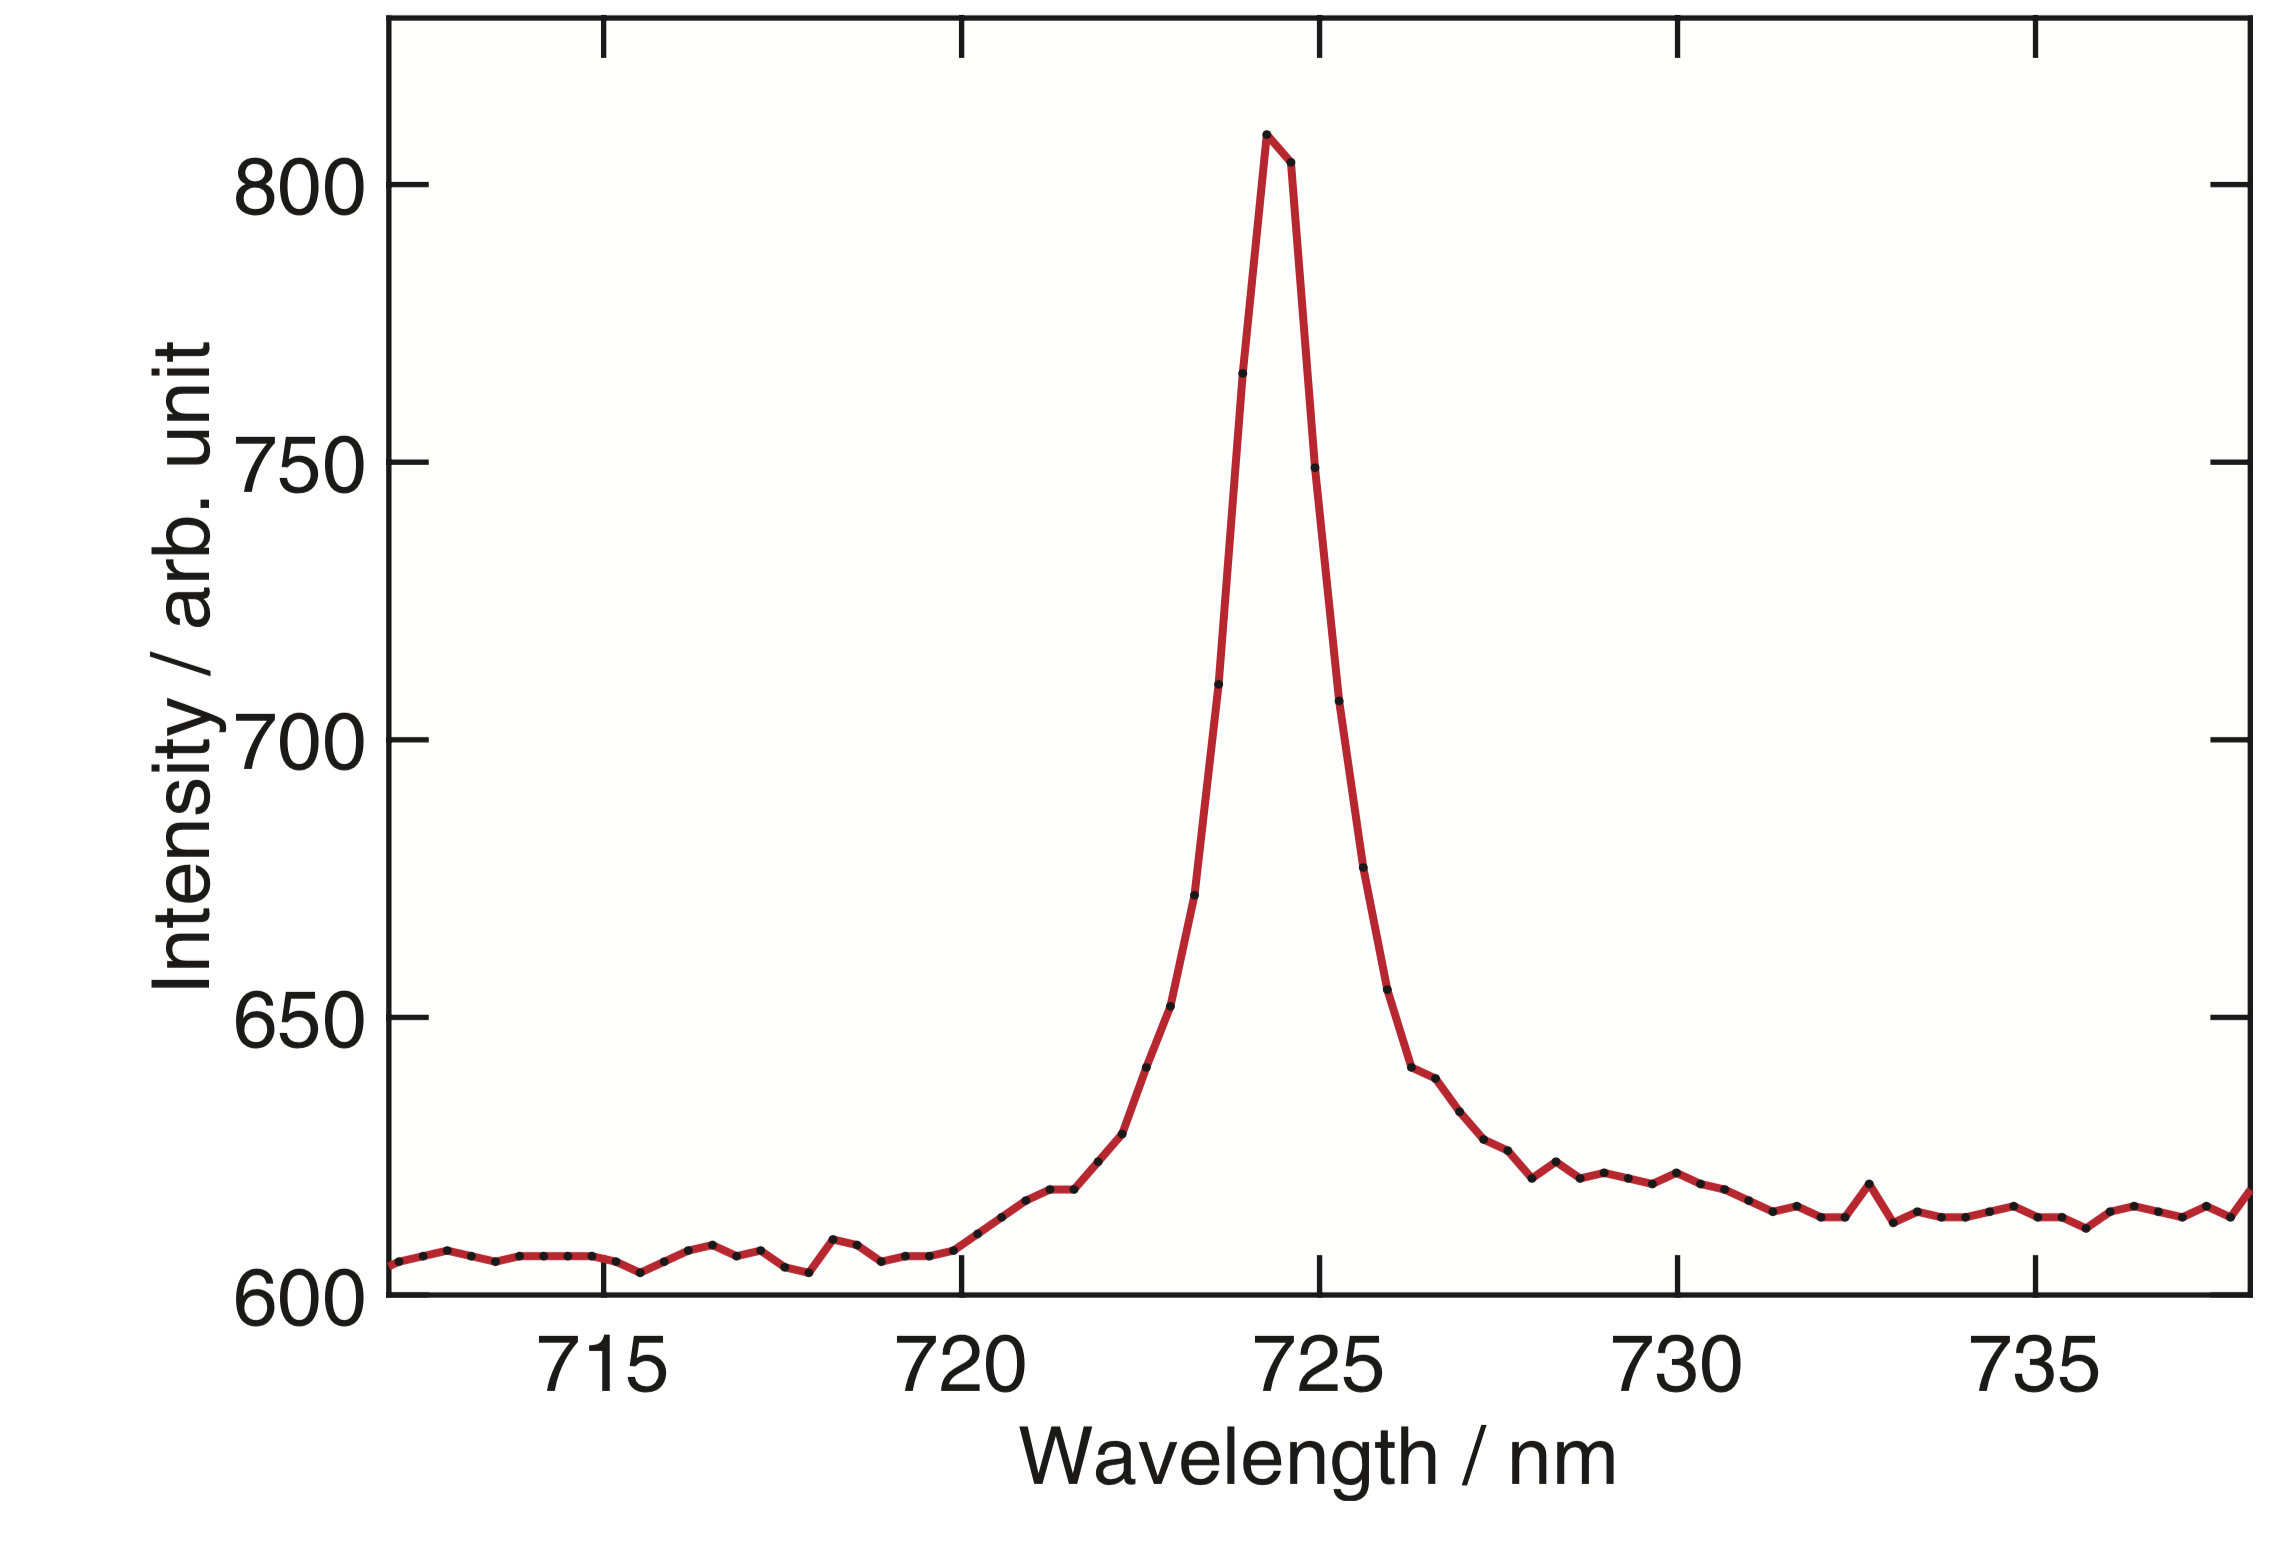
\includegraphics[trim = 0 0 0 0,  clip= true, width = \pairplotwide]{./pics/spectrum_erlangen_publication.png}}
				\caption{}
				\label{subfig::erlangen_spectrum}
			\end{subfigure}
			\hfill
			\begin{subfigure}[t]{ 0.49\linewidth}
				\centering
				\testbox{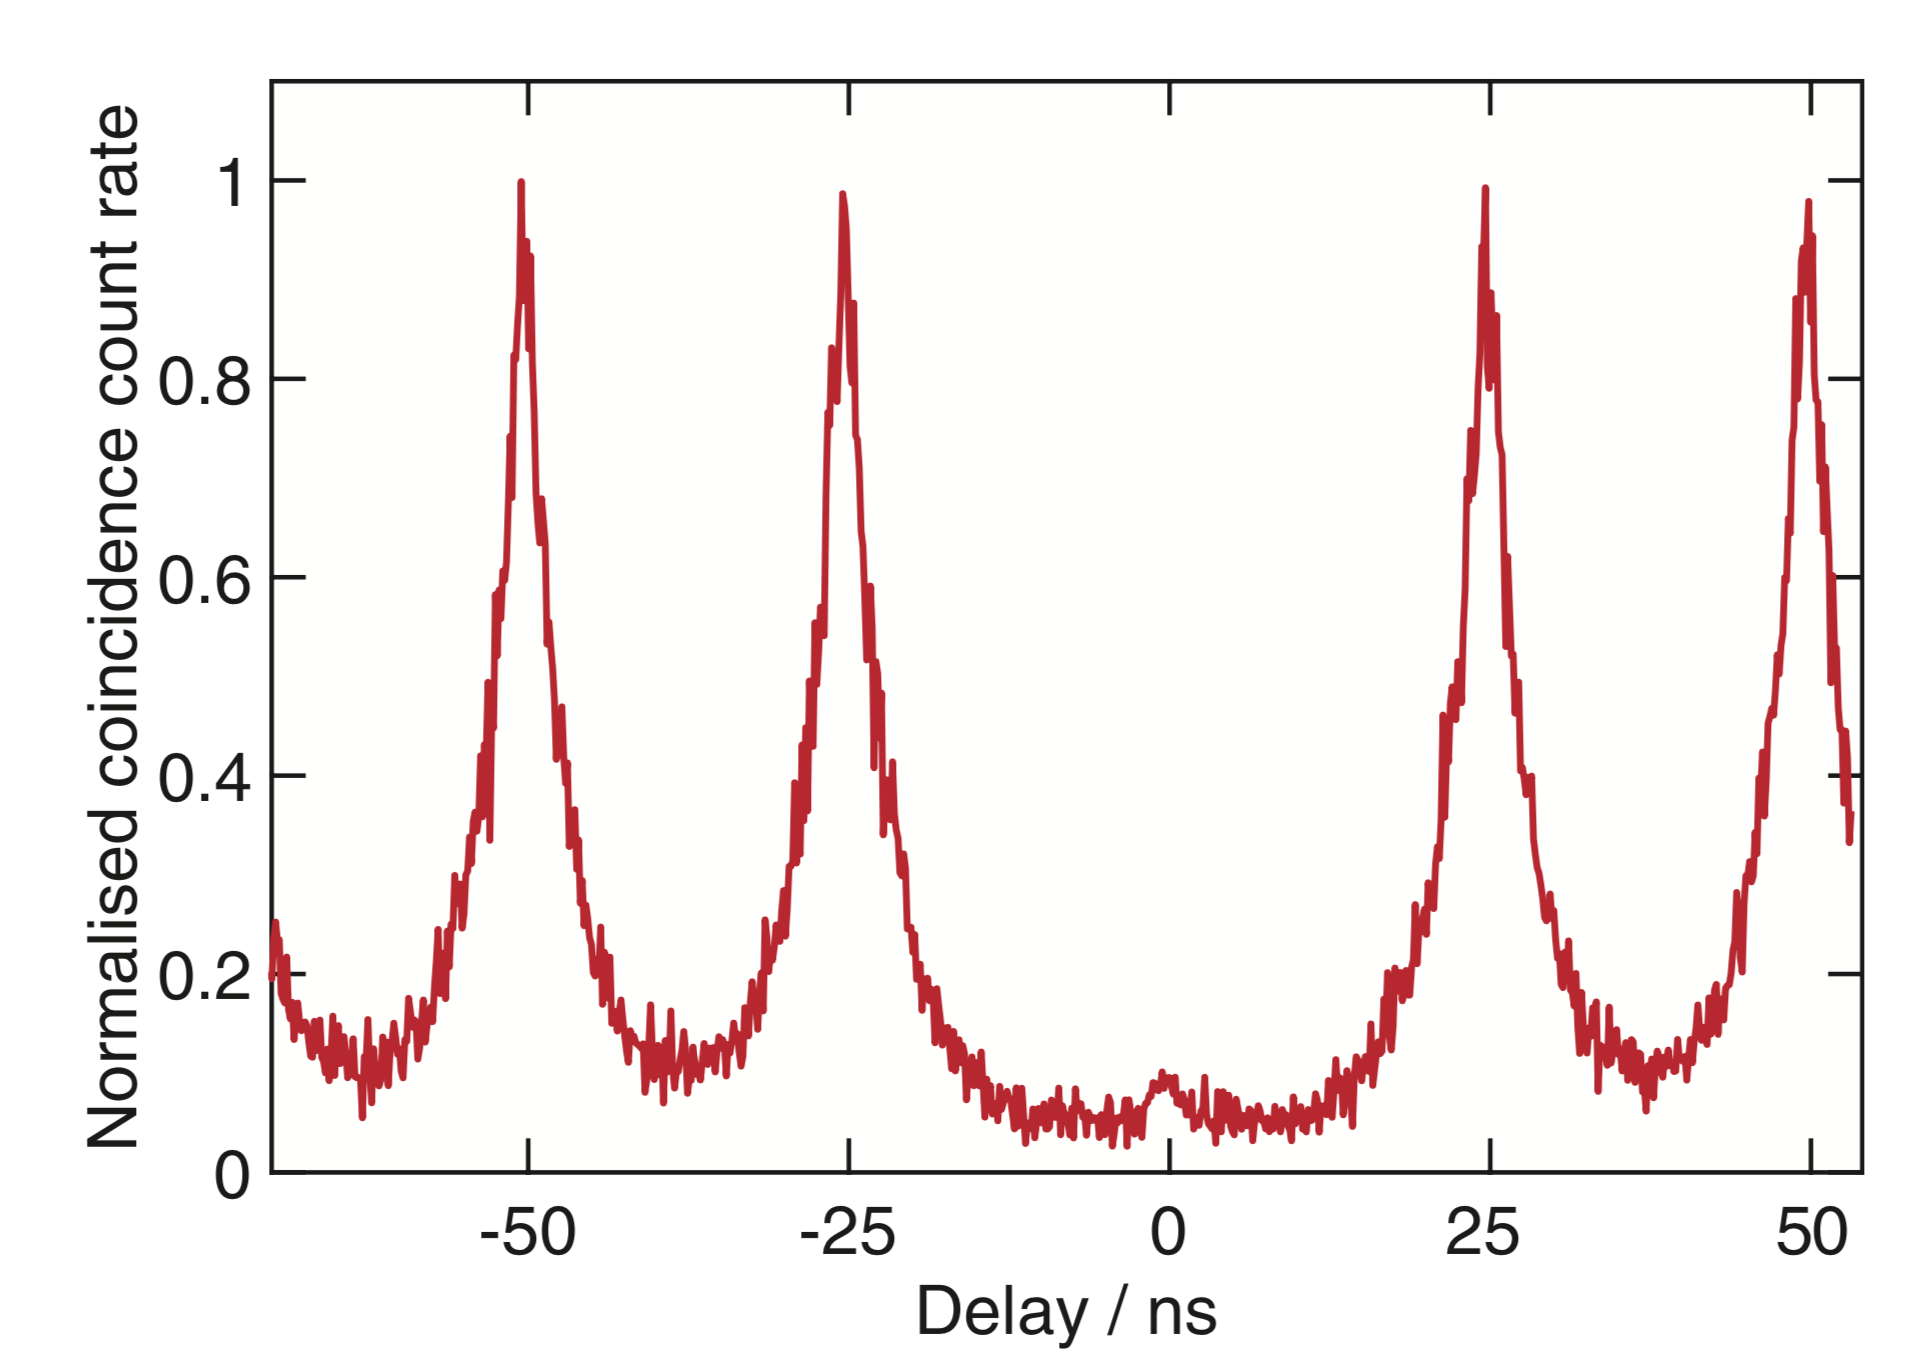
\includegraphics[trim = 0 0 0 0,  clip= true, width = \pairplotwide]{./pics/g2_erlangen_publication.png}}
				\caption{}
				\label{subfig::erlangen_lifetime}
			\end{subfigure}
			\caption[Spectrum and pulsed \gtf of an emitter]{(a) Spectrum of emitter \emhtwo. The \cwl amounts to \SI{724}{nm} and the \lw to \SI{2.0}{nm}. (b) Pulsed \gtf of the same emitter. \gtz amounts to \num{0.2}. Figures reproduced from \cite{Vaigu2017}.}
			\label{fig::erlangen_spectrum_lifetime}
		\end{figure}

		\Fref{subfig::g2_a} shows the photon correlation function of \emhtwo under \cw excitation.
		The shift of the dip to $\tau=\SI{50}{ns}$ originates from a path length difference of the two detection paths in the \HBT setup.
		The \gtz value of the fit is \num{0.20}.
		\\
		We also performed measurements with a pulsed laser, which is a prerequisite for a direct link between the high photon flux levels of the classical regime and low photon flux levels in the quantum world \cite{Vaigu2017,SiquteProject}, as mentioned in \Fref{ch::introduction}.
		The pulsed second-order correlation at zero delay \gtz are calculated by integrating photon counts in the zero-time-delay peak and dividing by the average of the adjacent peaks.
		\\
		The excited state lifetime of the emitter was determined to be \SI[separate-uncertainty]{3.8\pm0.1}{ns}, see \Fref{fig::lifetime}.
		For this, the emitter is excited by a pulsed laser (PiL069XSM from Advanced Laser Diode Systems A.L.S. GmbH) produces short optical pulses of less than \SI{50}{\ps} at a maximum repetition rate of \SI{80}{\mega\hertz} and a wavelength of \SI{685}{\nm} \cite{Vaigu2017}. 
		The measured time intervals between the optical pulse and the detected \fl yields the exponentially decaying lifetime of the excited state.
		The lifetime of the emitter is the time interval after which the number of $N_0$ excited emitters decreases to $N_0/e$.
		
		\begin{figure}[!htb]
			\centering
			\testbox{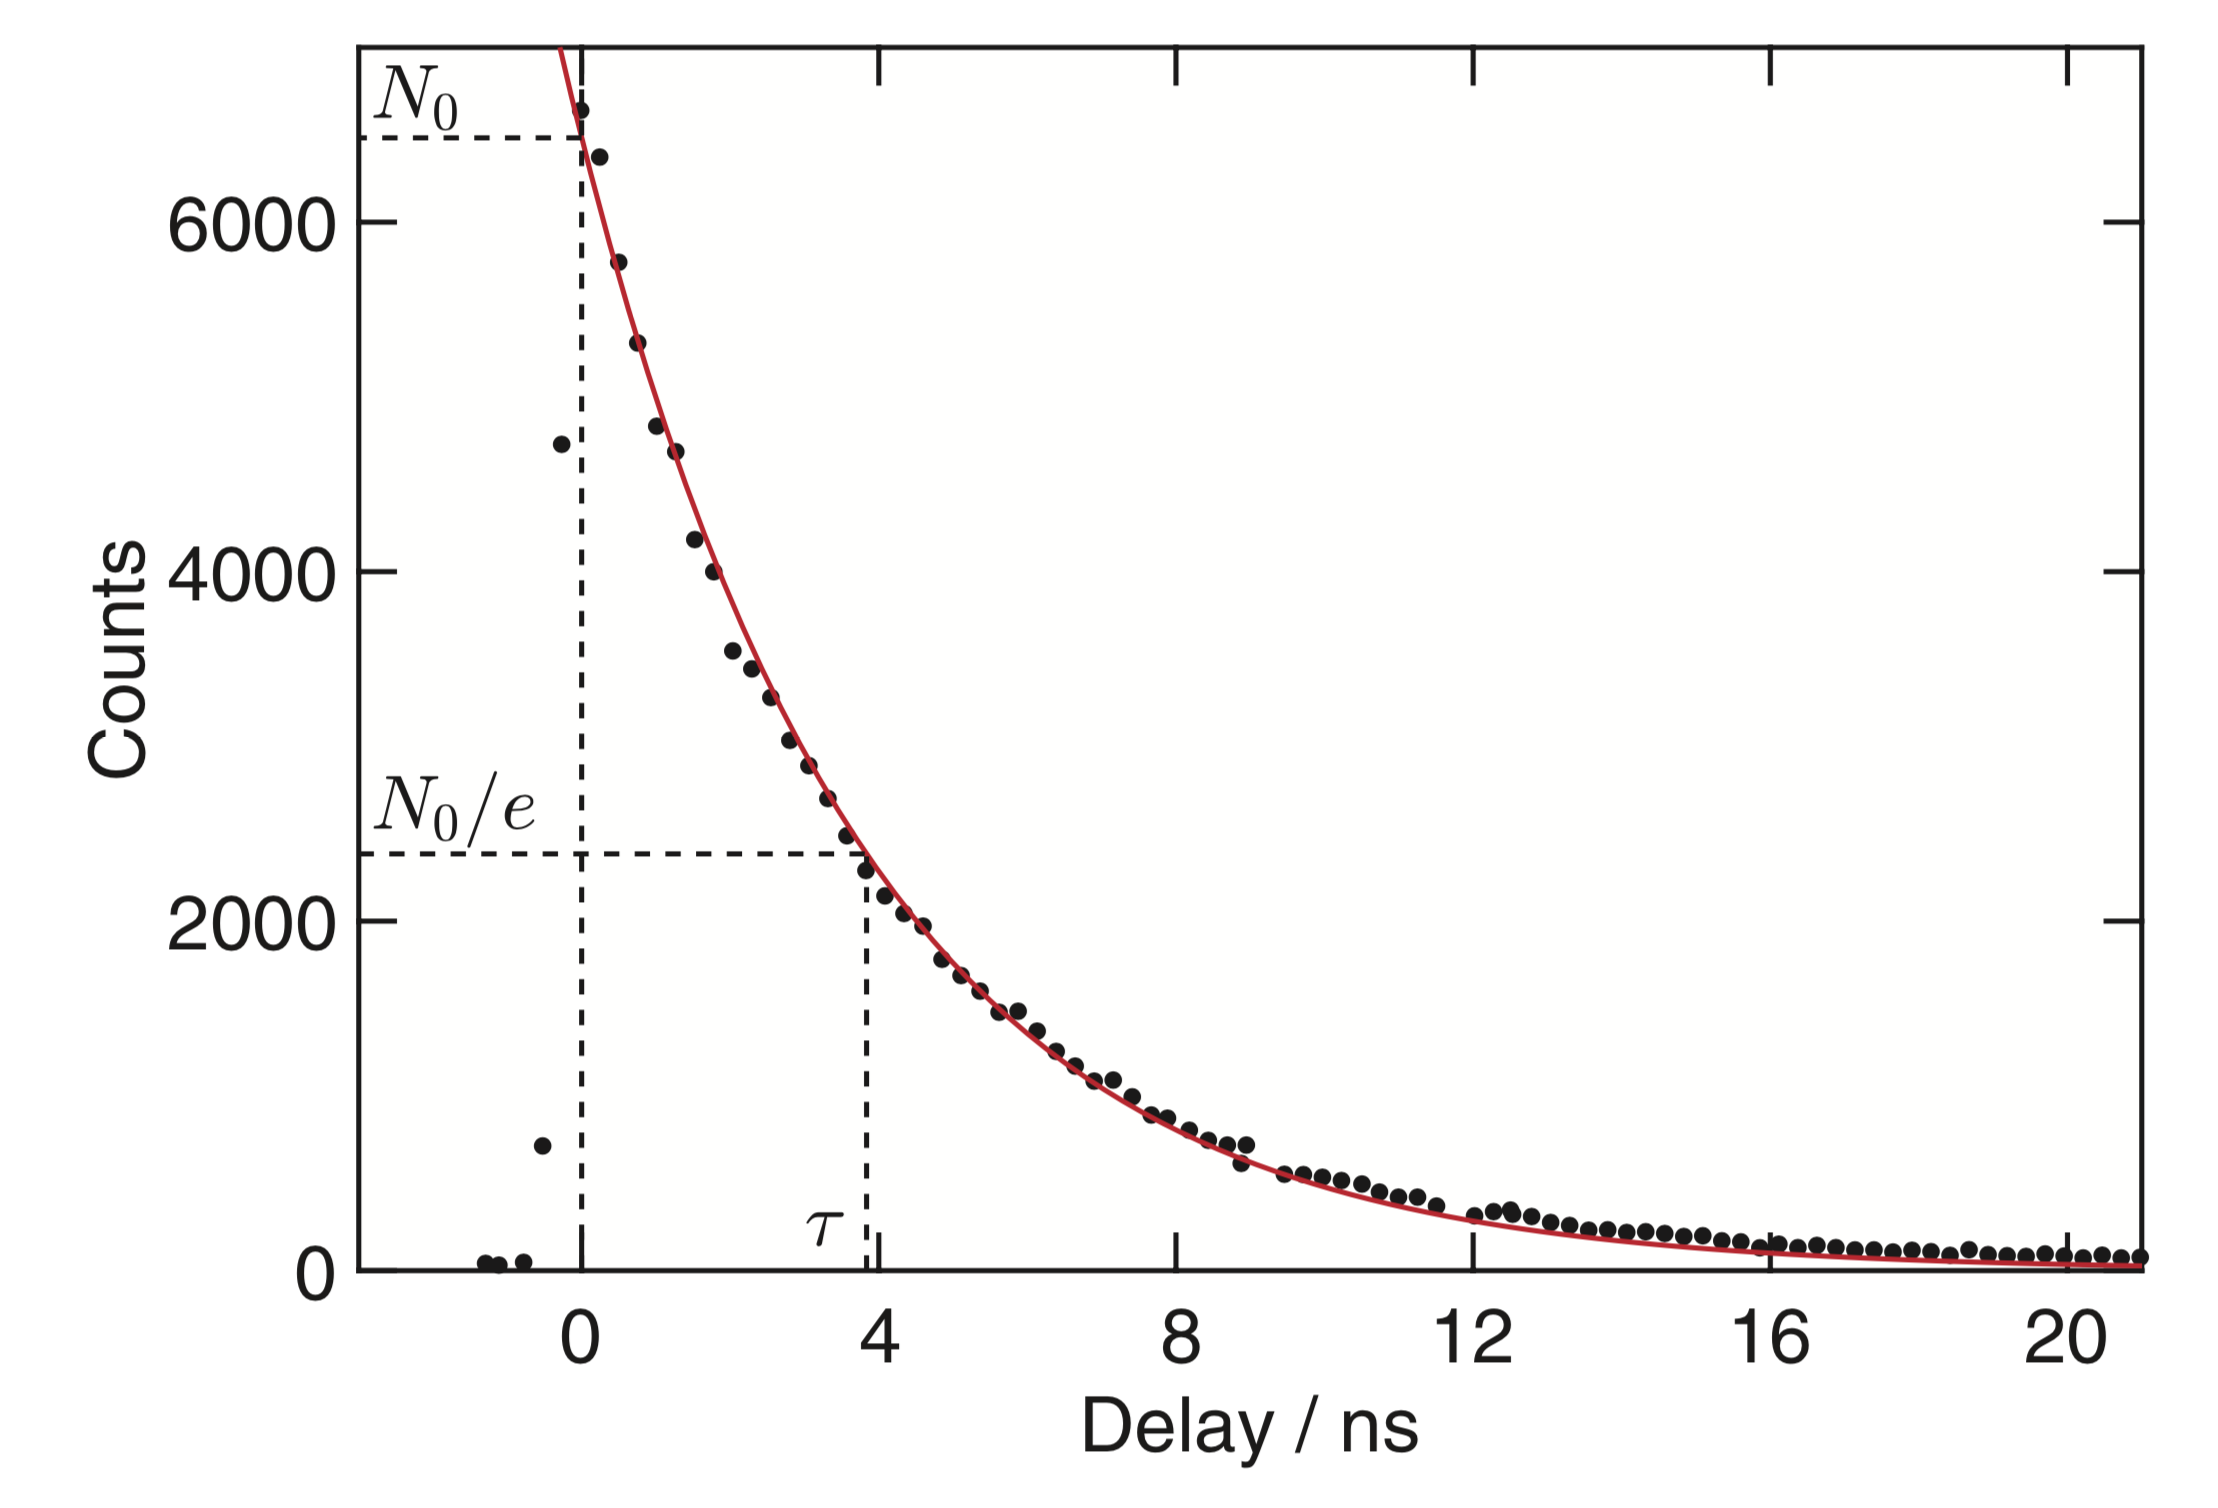
\includegraphics[trim = 0 0 0 0,  clip= true, width = 0.6\linewidth]{./pics/lifetime_erlangen_publication.png}}
			\caption[Lifetime measurement of an emitter]{Lifetime measurement of emitter \emhtwo. The lifetime of the emitter is the time interval after which the number of $N_0$ excited emitters decreases to $N_0/e$. Figure reproduced from \cite{Vaigu2017}.}
			\label{fig::lifetime}
		\end{figure}

		
		\begin{figure}[!htb]
			\centering
			\testbox{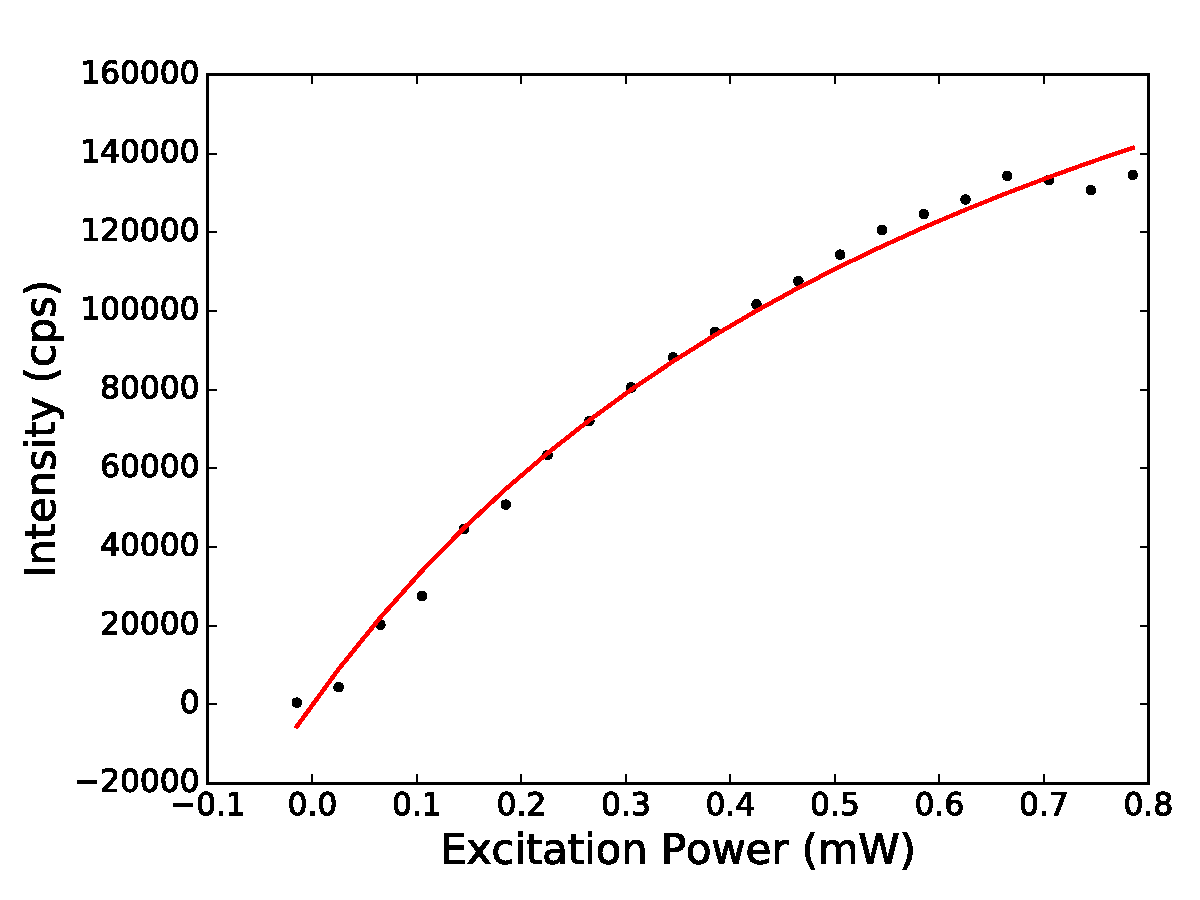
\includegraphics[trim = 0 0 0 0,  clip= true, width = 0.6\linewidth]{./pics/Ir8_sat_scan_xy-05_fit_notitle.pdf}}
			\caption[Saturation measurement of an emitter]{Saturation measurement of emitter \embroad.}
			\label{fig::sat_Ir8}
		\end{figure}

		An important characteristic of \spss is their photon count rate at saturation. The count rate $I(P)$ as a function of the excitation power $P$ is given by
		% 
		\begin{equation}
			I(P) = I_{\infty} \frac{P}{P + P_{sat}} + c_b P.
		\end{equation}

		Here $I_{\infty}$ refers to the maximal photon count rate, while the saturation power is denoted by $P_{sat}$. These two quantities are parameters determined by fitting count rates $I(P)$ measured at different excitation powers $P$. The added term $c_b P$ takes into account the linear increase of background fluorescence from the diamond host material at higher excitation powers. When background effects are negligible, this term can be omitted.

		\Fref{fig::sat_Ir8} depicts the saturation curve of \embroad.
		The saturation count-rate amounts to \SI[separate-uncertainty]{340\pm20}{cps} at a saturation power of \SI[separate-uncertainty]{1.0\pm0.1}{mW}.
		\Fref{subfig::g2_b} shows the \gt function of \embroad at an excitation power of \SI{200}{\micro\W}, which is \SI{20}{\percent} of the emitter's saturation power $P_{sat}=\SI[separate-uncertainty]{1.0\pm0.1}{mW}$.
		The \gtz value yields \num{0.16}.
		It is a \gt measurement representative of single \sivs.
		It is well below \num{0.5}, indicating single photon emission.
		The non-vanishing \gtz value is caused by background fluorescence of the diamond.
		The lifetime of the excited state of this emitter is \SI[separate-uncertainty]{9.2\pm0.2}{ns}.
		It is the highest excited state lifetime we measured within this work.
		\\
		Several \nd \pl spectra contain multiple narrow distinct peaks at different \wls.
		This circumstance is attributed to \nds containing more than one \siv, each of which is subject to a different \ZPL \wl shift.
		We choose narrow bandpass filters to perform independent measurements of each individual peaks of such a spectrum.
		As a result it is possible to measure \gtz values below \num{0.5} for each of these narrow peaks.
		Hence the individual peaks are identified as single emitters with a different ZPL \cwl.
		\\
		We do not see a systematic difference regarding the photon autocorrelation functions of \hl and \vl, both reach similar \gtz values.
		Also, the timescales of the excited state lifetimes coincide.
